\section{Theory}

\subsection{Background}

\begin{frame}
    \frametitle{Markov Decision Process (MDP)}
    
    Framework for modeling decision making in partly random processes.\\
    In our case, \textit{partially observable} MDP~\cite{kaelbling_planning_1998}:

    \begin{itemize}
        \item \textit{Agent} interacts with \textit{environment} over discrete time steps \(t = 0, 1, 2\dots, T\).
        \item Takes \textit{action} \(a_t\) in state \(s_t\).
        \item Perceives (partial) \textit{observation} of state \(o_t\).
        \item Receives scalar reward \(r_t\) that indicates whether action is good or bad.
        \item New state \(s_{t+1}\) depends only on history of interactions.
        \item Agent usually maintains some internal state depending on history \\
        \(\rightarrow\) memory.
    \end{itemize}

    \begin{figure}
        \centering
        \scalebox{0.75}{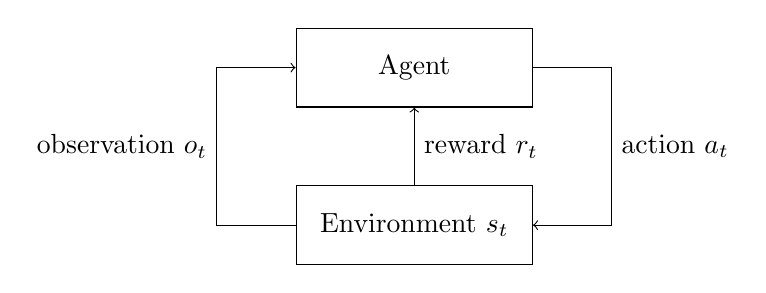
\begin{tikzpicture}[node distance=2cm]
    \tikzstyle{block} = [rectangle,minimum width=3cm,minimum height=1cm,text centered,draw=black,fill=white]
    \node (agent)[block]{Agent};
    \node (environment)[block,below of=agent]{Environment \(s_t\)};
    \draw [->] (agent.east) -- ++(1cm,0) -- node [anchor=west]{action \(a_t\)} ++(0,-2cm) -- (environment.east);
    \draw [->] (environment.north) -- node [anchor=west]{reward \(r_t\)} (agent.south);
    \draw [->] (environment.west) -- ++(-1cm,0) -- node [anchor=east]{observation \(o_t\)} ++(0,+2cm) -- (agent.west);
\end{tikzpicture}}
    \end{figure}
\end{frame}

\begin{frame}
    \frametitle{Reinforcement Learning (RL)}

    Paradigm for learning from interactions how to achieve a goal.

    \begin{itemize}
        \item Tasks usually formalized as (partially observable) MDPs.
        \item Policy \(\pi(a|s)\) is a mapping from states to action probabilities.
        \item Find \(\pi\) that maximizes cumulative reward \(\mathbb{E} \left\lbrack \sum_{k=0}^{T} \gamma^{k-t-1} r_k \right\rbrack\).
        \item Often involves estimating the value \(v_\pi(s)\) of a state under policy \(\pi\) (useful for training). 
    \end{itemize}

    Deep RL: Approximate \(\pi\) (and \(v_\pi\)) with deep neural networks.
    Has been used to play Atari~\cite{mnih_human-level_2015}, Go~\cite{silver_mastering_2016}, StarCraft II~\cite{vinyals_grandmaster_2019}, etc.
\end{frame}

\begin{frame}
    \frametitle{Proximal Policy Optimization}

    
\end{frame}

\subsection{Related Work}

\begin{frame}
    \frametitle{Related Work}

    Deep RL for active vision tasks:

    \begin{itemize}
        \item Visual attention:
        \begin{itemize}
            \item Sequential focus points for foveated vision~\cite{mnih_recurrent_2014}.
        \end{itemize}
        \item Visual navigation:
        \begin{itemize}
            \item Solve random mazes~\cite{mirowski_learning_2017}.
        \end{itemize}
        \item Object detection:
        \begin{itemize}
            \item Region proposals for object localization~\cite{caicedo_active_2015}.
            \item Contextual reasoning over spatial layout in scenes~\cite{chen_spatial_2017}.
            \item Anatomical landmark detection in medical images~\cite{ghesu_multi-scale_2019}.
        \end{itemize}        
    \end{itemize}
\end{frame}